\documentclass[11pt]{article}
\usepackage{physics}
\usepackage{bm}
\usepackage[font=scriptsize]{caption}
\usepackage{graphicx}

\begin{document}
This repository contains training data for an ML-based parameter optimization for modeling morphogen gradient formation by a source-diffusion-sink (SDS) mechanism~\cite{Yu2009}, as described by the following one-dimensional (1D) reaction-diffusion partial differential equation:

\begin{equation}\label{eq:SDS_1D_PDE}
	\frac{\partial c(x,t)}{\partial t} = f_{\rm{source}}(x) + D\frac{\partial^2 }{\partial x^2}c(x,t) - k_{\rm{sink}}c(x,t)\,.
\end{equation}

Here, $c(x,t)$ is the scalar concentration field of the morphogen in space $x$ at time $t$, $D$ is the constant homogeneous diffusion coefficient, $k_{\rm{sink}}$ is the sink rate scaling with $c(x,t)$, describing morphogen degradation by the cells and proteases in the extracellular space, and $f_{\rm{source}}$ is the source term describing morphogen secretion by the source cells. 

$f_{\rm{source}}$ depends on the location as only a group of cells produce the morphogen, i.e.,
\begin{equation}\label{eq:source}
	f_{\rm{source}}(x) =
        \begin{cases}
        k_{\rm{source}} \quad & \text{for} \quad x | d_{\rm{margin}}(x) \le w_{\rm{source}}  \\
        0 & \rm{otherwise}\, 
    \end{cases}  
\end{equation}
%
in a 1D diffusion domain $\Omega = \{x | -\frac{L}{2} \leq x \leq \frac{L}{2}\}$ of length $L=2.0$. The source is a region of width $w_{\rm{source}} = 0.3 L$ restricted to a distance $d_{\rm{margin}}(x) \le w_{\rm{source}}$ from the left margin. We consider the scenario of a zero morphogen concentration in $\Omega$ as initial condition
%
\begin{equation}\label{eq:IC}
	c(x,0) = 0, \quad x \in \Omega
\end{equation}
%
and homogeneous zero-flux Neumann boundary conditions at all boundaries $\partial \Omega$, i.e.,
%
\begin{equation}\label{eq:no_flux_BCs}
    \left. \frac{\partial c(x, t)}{\partial \bm n} \right\rvert_{x \in \partial \Omega} = 0\,,
\end{equation}
with $\bm n$ as the normal vector on $\partial \Omega$. We discretize $\Omega$ by 64 grid points, resulting in a grid spacing of $\Delta x=0.031746$. The timestep size depends on $\Delta x$ and the diffusion coefficient as
%
\begin{equation}{\label{eq:diffusion_stability_condition}}
    \Delta t = \frac{1}{8  D}  \Delta x^{2}\, .
\end{equation}
%
We solve Eq.~\eqref{eq:SDS_1D_PDE}--\eqref{eq:diffusion_stability_condition} using first-order forward-time central-space finite differences until Eq.~\eqref{eq:SDS_1D_PDE} reaches a steady-state. This steady-state morphogen concentration profile can be flat, exponential, or step-wise depending on the parameters $k_{\rm{source}}$, $k_{\rm{sink}}$, and $D$. The goal is to generate a model that predicts a parameter set given an input gradient. To train this model, we produce simulated training data by solving Eq.~\eqref{eq:SDS_1D_PDE} until steady-state for different parameter sets.

The output folders contain a parameters.csv file, where the first row defines the parameter type of the respective column, and each row below contains a set of parameters with index $i$ (see Fig.~\ref{fig:description_csv_files}). The corresponding gradients folder contains gradient\_$i$.csv files, each corresponding to one row $i$ of the parameters.csv file. The columns of gradient\_$i$.csv contain the concentration value at each grid point and each row contains one iteration, as shown in Fig.~\ref{fig:description_csv_files}.

\begin{figure}[htbp!]
\footnotesize
    \centering
    \captionsetup{width=1.0 \textwidth}
    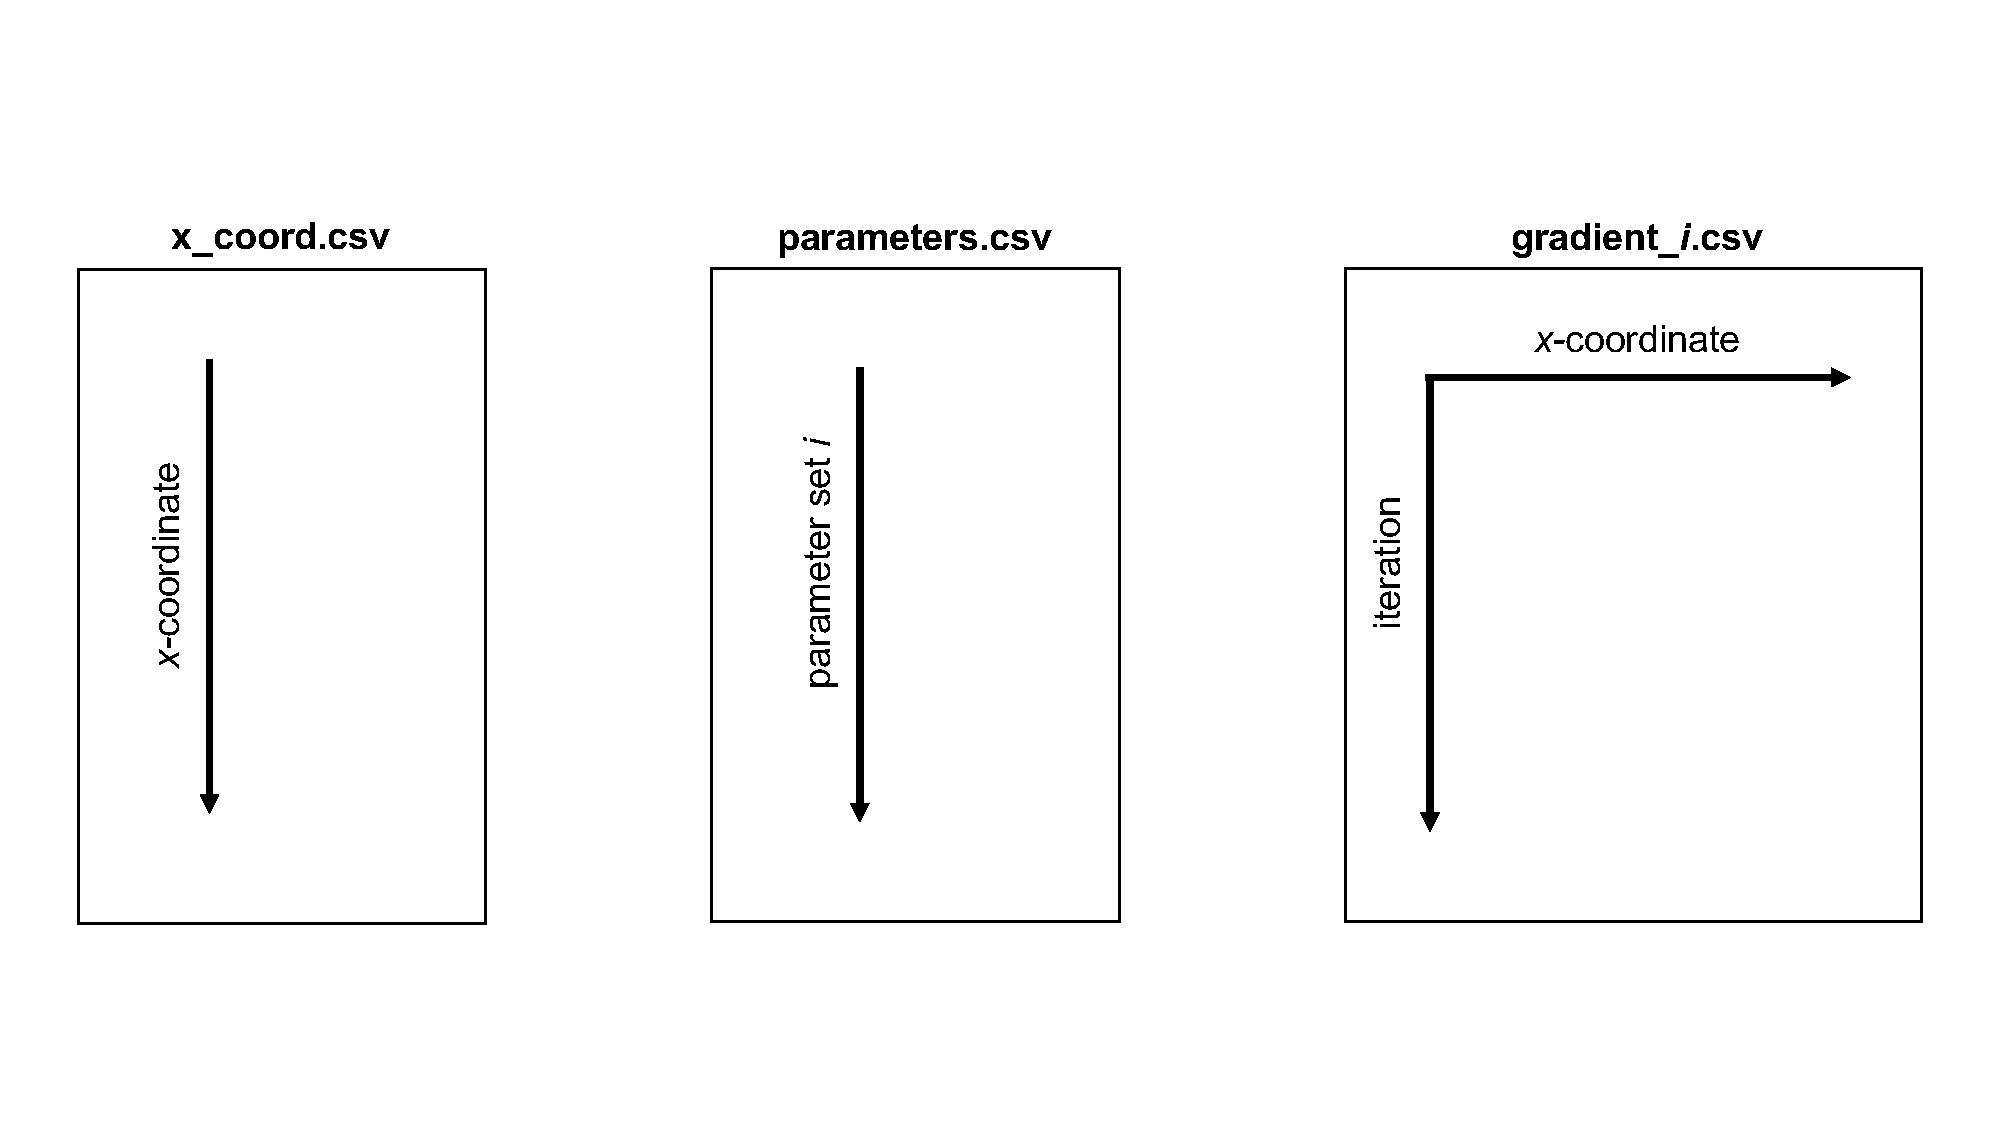
\includegraphics[width=1.0\textwidth]{./description_csv_files.pdf}
    \caption{}
\label{fig:description_csv_files}
\end{figure}
%\FloatBarrier


Each gradient\_$i$.csv file contains two columns: the first containing $x$, the second containing the steady-state concentration field $c(x, t_{\rm{max}})$.


\begin{thebibliography}{9}
 \bibitem{Yu2009} \textsc{S. R. Yu, M. Burkhardt, M. Nowak, J. Ries, Z. Petr\'a\v{s}ek, S. Scholpp, P. Schwille and M. Brand}. Fgf8 morphogen gradient forms by a source-sink mechanism with freely diffusing molecules.
  \emph{Nature} \textbf{volume}(461),
  533--536, 2009.	
\end{thebibliography}
\end{document}
